\documentclass{article}
\usepackage{iclr2026_conference,times}
\input{math_commands.tex}
\usepackage{hyperref}
\hypersetup{hidelinks}
\usepackage{url}
\usepackage{booktabs}
\usepackage{graphicx}
\usepackage{amsmath}
\usepackage{amssymb}
\usepackage{microtype}

\title{Posterior-Tail Selection in Bayesian Ensemble World Models}

\author{Anonymous Authors\\
Paper under double-blind review}

\newcommand{\PaperSeeds}{5}
\newcommand{\PaperProblems}{225}
\newcommand{\PaperHighN}{128}
\newcommand{\PaperLowN}{2}
\newcommand{\MeanHighTrue}{16.355}
\newcommand{\MeanHighRegret}{0.100}
\newcommand{\SampleHighTrue}{5.567}
\newcommand{\ThompsonHighTrue}{11.895}
\newcommand{\UcbHighTrue}{16.058}
\newcommand{\PessHighTrue}{16.223}
\newcommand{\OracleHighTrue}{16.455}
\newcommand{\SampleHighRegret}{10.888}
\newcommand{\PessHighRegret}{0.233}
\newcommand{\SampleHighOptimism}{0.459}
\newcommand{\PessHighOptimism}{-1.233}
\newcommand{\SampleHighStd}{8.234}
\newcommand{\SampleHighSampleGap}{13.726}
\newcommand{\SampleHighOOD}{0.304}
\newcommand{\PessHighOOD}{0.168}
\newcommand{\SampleHighTail}{0.276}
\newcommand{\PessHighTail}{0.004}
\newcommand{\SampleLowTrue}{1.952}


\begin{document}
\maketitle

\begin{abstract}
Bayesian and ensemble world models expose epistemic uncertainty, so they are
often treated as a safer substrate for planning. This paper studies a failure
in how that uncertainty is consumed: score each candidate trajectory with a
posterior-sampled model member, execute the candidate with the largest sampled
score, and the selector can convert epistemic uncertainty into a selected
upper-tail residual. We call this failure \emph{posterior-tail selection}. In a
controlled latent dynamics benchmark with \PaperSeeds{} posterior seeds and
\PaperProblems{} candidate problems, sampled-posterior max selection at
$N=\PaperHighN{}$ reaches true return \SampleHighTrue{} and regret
\SampleHighRegret{} to the in-set candidate oracle, while posterior-mean
selection reaches true return \MeanHighTrue{} and regret \MeanHighRegret{}. The selected
sampled-posterior trajectory has posterior standard deviation \SampleHighStd{},
sample-over-mean residual \SampleHighSampleGap{}, OOD mass \SampleHighOOD{}, and hazard-tail
selection rate \SampleHighTail{}. A calibration-aware lower-confidence selector
reduces regret to \PessHighRegret{} and tail selection to \PessHighTail{} while
retaining most of the candidate-oracle value. The contribution is intentionally
narrow: a mechanism, diagnostic benchmark, and repair for posterior-tail
aggregation in Bayesian or ensemble world-model rollouts, not a claim of
real-robot or large-scale benchmark dominance.
\end{abstract}

\section{Introduction}

World models let agents evaluate futures before acting. Modern systems learn latent dynamics for planning and policy learning \citep{hafner2019planet,hafner2020dreamer,hafner2023dreamerv3}, use ensembles to represent model uncertainty \citep{chua2018pets,lakshminarayanan2017deep}, and often combine learned models with model-predictive control or offline policy optimization \citep{janner2019mbpo,yu2020mopo,kidambi2020morel,yu2021combo}. A common deployment instinct is to spend more inference-time compute: sample $N$ candidate action sequences, roll them out in the world model, and choose the best.

This paper asks what happens when the deployment score is not a posterior mean
or lower confidence bound, but a separately sampled posterior value for each
candidate. The rule resembles Thompson sampling locally, but the many-candidate
maximum changes its behavior: a candidate can win because one plausible model
member hallucinates high return in an epistemically uncertain region. The agent
then executes a trajectory that is not robust under the posterior.

The phenomenon is related to reward-model overoptimization in language models \citep{gao2023scaling,jinnai2024regularized,huang2025bon,yu2026caution,hsu2026tails}. The difference is architectural. In Bayesian world models, the error source is a learned dynamics posterior over imagined trajectories, and the diagnostic should measure trajectory OOD mass, ensemble dispersion, and posterior sample-over-mean gaps.

We contribute:
\begin{itemize}
    \item the posterior-tail selection failure mode for Bayesian and ensemble
    world-model planning;
    \item a compact selected-residual proposition showing why a maximum over
    posterior-sampled scores exposes upper-tail model error;
    \item a deterministic latent dynamics benchmark for posterior-sampled and
    ensemble world-model selectors;
    \item selected-trajectory diagnostics for OOD mass, hazard mass, ensemble
    dispersion, sampled residual, and regret to the in-set candidate oracle;
    \item a calibration-aware lower-confidence repair that uses held-out
    residual calibration and test-time ensemble predictions only.
\end{itemize}

\section{Mechanism}

Let $a_1,\ldots,a_N$ be candidate action sequences. A Bayesian or ensemble
world model gives each candidate a posterior distribution over imagined
returns. Write a posterior sample score as
\begin{equation}
    S_i = \mu_i + \epsilon_i,
\end{equation}
where $\mu_i$ is the posterior mean and $\epsilon_i$ is the sampled
model-member residual. The sampled-posterior max selector chooses
$\hat{i}=\arg\max_i S_i$.

\paragraph{Diagnostic proposition.}
Suppose $\epsilon_i$ are independent centered residuals conditional on the candidate set, and suppose at least two candidates have nonzero residual variance. Then
\begin{equation}
    \mathbb{E}\left[\epsilon_{\hat{i}}\right] \geq 0,
\end{equation}
with strict inequality whenever residual variance can affect the argmax. Moreover, in equal-mean Gaussian residuals with variance $\sigma^2$, the expected selected residual scales as $\sigma \mathbb{E}[\max_i Z_i]$, which grows like $\sigma\sqrt{2\log N}$.

This is not a theorem about all learned controllers. It is a warning about the
aggregation operator. Posterior sampling is useful for exploration when one
sampled model is followed coherently. A maximum over independently sampled
trajectory scores instead searches for posterior outliers.

\paragraph{Repair principle.}
Use a posterior-robust score:
\begin{equation}
    L_i = \mu_i - \beta \sigma_i,
\end{equation}
where $\sigma_i$ is ensemble standard deviation and $\beta$ is fitted from held-out calibration candidates as a high quantile of $|\mu_i - V_i| / (\sigma_i+\epsilon)$. This is deliberately simple: the paper tests whether the selected-tail failure is visible enough that a scalar lower-confidence rule removes it.

\section{Benchmark}

We build a two-dimensional latent control system with position and velocity. The true dynamics reward approaching a goal region and penalize entering a high-position hazard. Candidate action sequences are smooth random controls with occasional high-excursion probes. The posterior ensemble is accurate near the training-like region but uncertain about hazard strength and terminal value in high-position regions.

For every problem instance, we draw a shared candidate set of size $\PaperHighN{}$ and evaluate smaller budgets by prefixing the same set. This makes curves across $N$ comparable. The selectors are:

\begin{itemize}
    \item \textbf{Posterior mean}: choose the candidate with largest ensemble mean.
    \item \textbf{Sampled-posterior max}: choose the largest score after sampling one ensemble member per candidate.
    \item \textbf{Thompson-member max}: choose a single model member and rank all candidates by that member.
    \item \textbf{Mean + std}: an optimistic upper-confidence selector.
    \item \textbf{Quantile and calibrated LCB}: posterior-pessimistic repairs.
    \item \textbf{Oracle}: choose the highest true return within the same candidate set.
\end{itemize}

The full sweep uses \PaperSeeds{} posterior seeds and \PaperProblems{} candidate problems. The code writes all detailed rows to \texttt{results/full/results.csv}; the paper figures are generated from \texttt{results/full/summary.csv}.

\section{Results}

\begin{figure}[t]
    \centering
    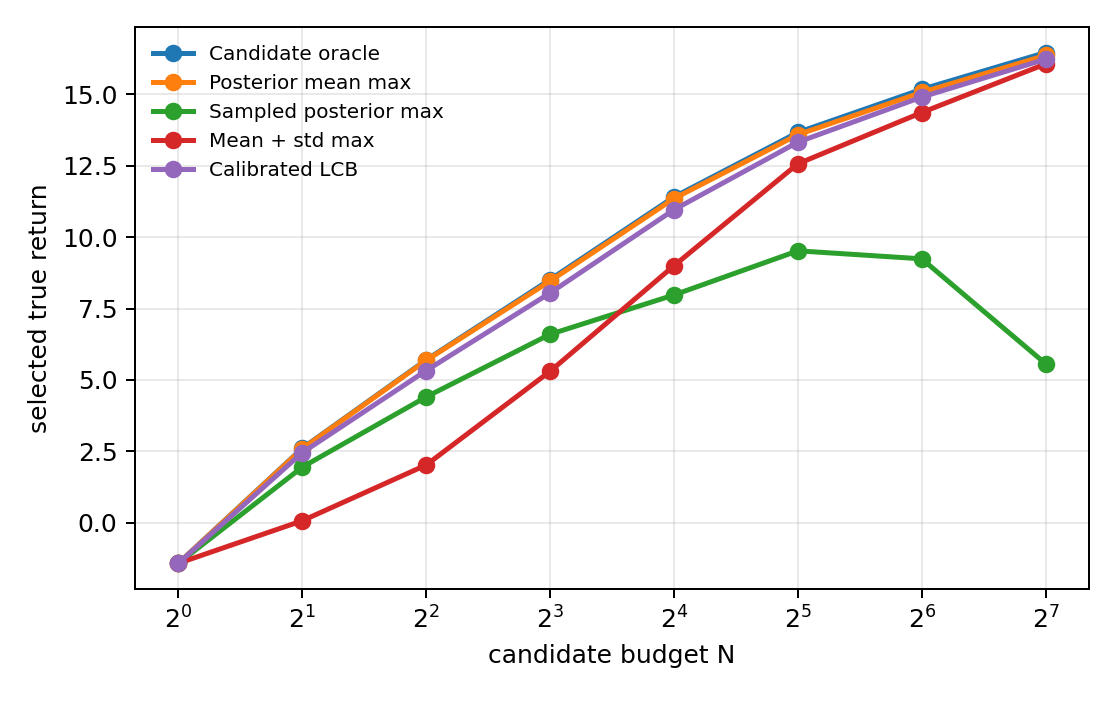
\includegraphics[width=0.49\linewidth]{../figures/full/true_return_vs_n.png}
    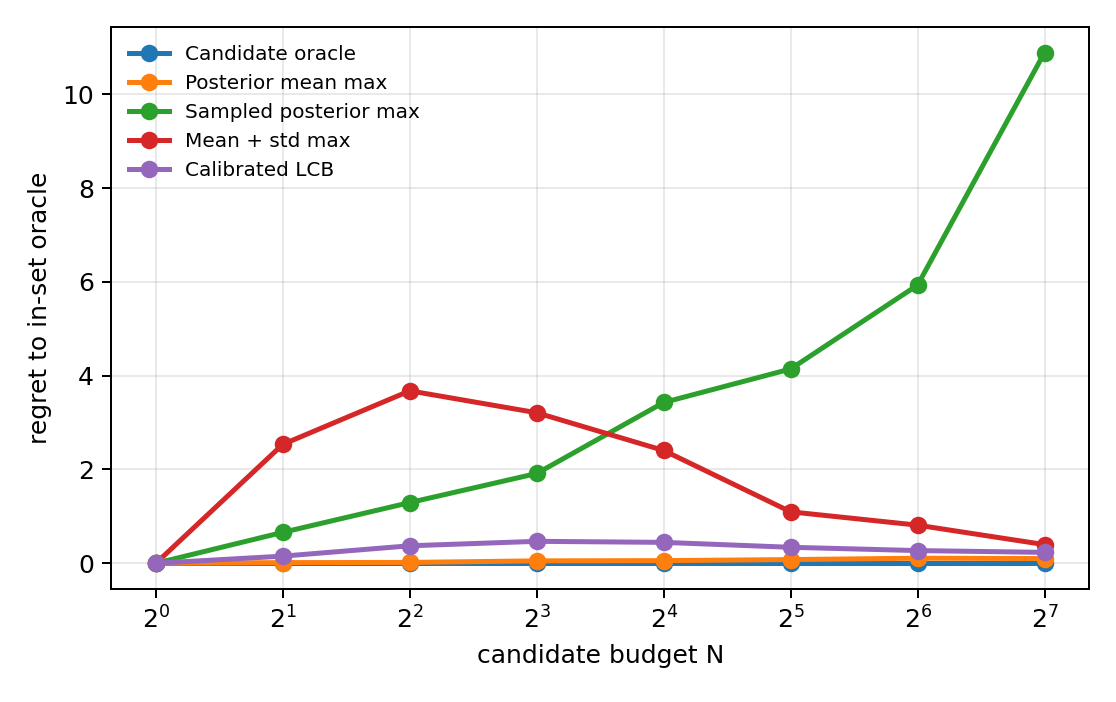
\includegraphics[width=0.49\linewidth]{../figures/full/regret_vs_n.png}
    \caption{Left: selected true return. Right: regret to the best true-return candidate in the same sampled set. Sampled-posterior max selection degrades at large $N$ despite the candidate set containing strong trajectories.}
    \label{fig:return}
\end{figure}

Figure~\ref{fig:return} shows the main result. At $N=\PaperHighN{}$, sampled-posterior max reaches true return \SampleHighTrue{} with regret \SampleHighRegret{}. Posterior mean reaches \MeanHighTrue{} with regret \MeanHighRegret{}, and the candidate oracle reaches \OracleHighTrue{}. The failure is therefore not lack of good candidates; it is the posterior-sampled selection rule.

\begin{figure}[t]
    \centering
    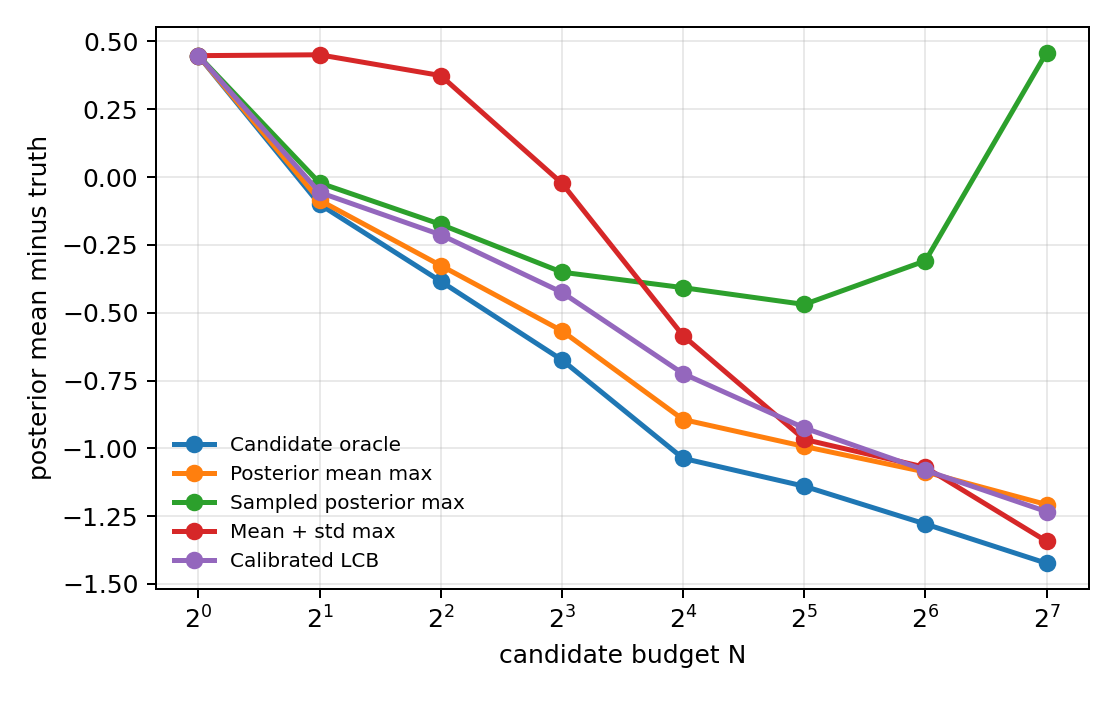
\includegraphics[width=0.49\linewidth]{../figures/full/optimism_gap_vs_n.png}
    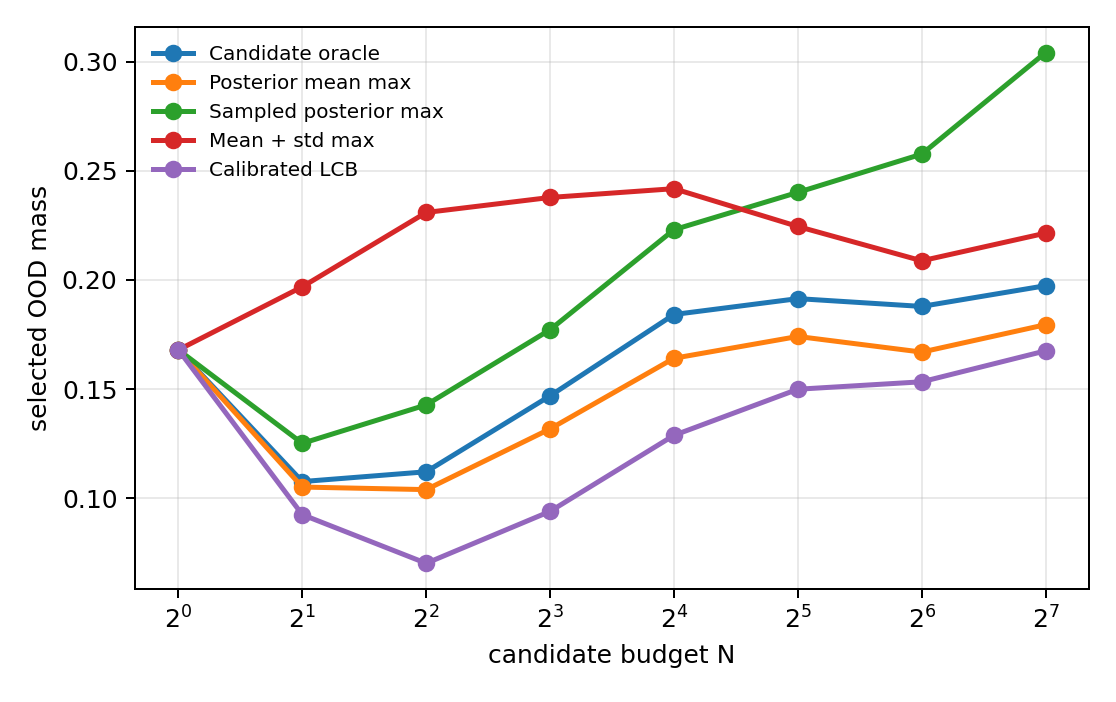
\includegraphics[width=0.49\linewidth]{../figures/full/uncertainty_exploitation_vs_n.png}
    \caption{Selected-trajectory diagnostics. Sampled-posterior max selection chooses candidates with higher OOD mass and large sampled-score residuals over the posterior mean.}
    \label{fig:diagnostics}
\end{figure}

Figure~\ref{fig:diagnostics} explains the mechanism. The posterior-sampled winner has selected OOD mass \SampleHighOOD{}, posterior standard deviation \SampleHighStd{}, and sampled score \SampleHighSampleGap{} above its posterior mean at $N=\PaperHighN{}$. In contrast, calibrated pessimism has selected OOD mass \PessHighOOD{} and tail-selection rate \PessHighTail{}. The lower-confidence repair obtains true return \PessHighTrue{} and regret \PessHighRegret{}.

Posterior mean is slightly better than calibrated pessimism in this benchmark.
This is a useful boundary: the paper is not claiming that pessimism always
improves over posterior means. It claims that if a deployment system uses
posterior-sampled or upper-tail ensemble scores for many-candidate planning, it
should audit selected residuals and consider lower-confidence aggregation.

\section{Related Work}

\paragraph{World models and ensemble planning.}
PlaNet and Dreamer learn latent dynamics for imagination and control \citep{hafner2019planet,hafner2020dreamer,hafner2023dreamerv3}. PETS introduced probabilistic ensembles with trajectory sampling for sample-efficient continuous control \citep{chua2018pets}. MBPO studies when short model rollouts are useful for policy optimization \citep{janner2019mbpo}. These works motivate the architecture, while our focus is the inference-time aggregation operator over posterior-sampled candidate scores.

\paragraph{Pessimism and model exploitation.}
MOPO, MOReL, COMBO, RAMBO, and CQL use pessimism or conservatism to avoid model or value overestimation in offline RL \citep{yu2020mopo,kidambi2020morel,yu2021combo,rigter2022rambo,kumar2020cql}. Our repair is much simpler and narrower: a calibrated lower-confidence score for a candidate selector.

\paragraph{Bayesian uncertainty.}
Deep ensembles, MC dropout, bootstrapped value functions, randomized priors, and posterior-sampling RL all provide uncertainty tools \citep{lakshminarayanan2017deep,gal2016dropout,osband2016bootstrapped,osband2018randomized,fan2021posterior}. Recent robotic world-model work also emphasizes epistemic uncertainty for deployment \citep{li2025rwm}. The current diagnostic asks how that uncertainty is consumed by many-candidate maximum selection.

\paragraph{Inference-time overoptimization.}
Reward-model overoptimization and inference-time alignment work show that
many-candidate selection can reward-hack imperfect learned scorers
\citep{gao2023scaling,jinnai2024regularized,huang2025bon,yu2026caution,hsu2026tails}.
We import the operator-level warning but specialize it to Bayesian ensemble
world models.

\section{Limitations}

This is a first-pass controlled benchmark. It does not show real-robot results, MuJoCo results, or large video world-model experiments. The synthetic posterior is hand-designed to expose an identifiable failure mode. The proposition assumes centered residuals and independence that are only approximations in learned dynamics. The repair is a scalar LCB rather than a conformal or task-adaptive uncertainty method. These limits are deliberate: the paper should be read as a falsifiable diagnostic and artifact, not as a final deployment recipe.

\section{Reproducibility and Ethics}

The repository includes code, tests, deterministic results, figures, literature notes, hostile-prior analysis, and a final audit. The benchmark is synthetic and has no human-subject data. The main safety implication is cautionary: increasing inference-time compute can amplify model error when the learned scorer is optimized too aggressively.

\bibliography{references}
\bibliographystyle{iclr2026_conference}

\appendix
\section{Checklist}

\begin{itemize}
    \item \textbf{Claims}: The main claims are limited to the synthetic benchmark and the stated diagnostic proposition.
    \item \textbf{Code}: The source package is under \texttt{src}; experiments are in \texttt{experiments/run\_benchmark.py}.
    \item \textbf{Data}: All data are generated synthetically from fixed seeds.
    \item \textbf{Compute}: The full sweep runs on CPU in roughly one minute on the development machine.
    \item \textbf{Prior work}: The repo includes a 100+ entry related-work matrix and a hostile-prior document.
\end{itemize}

\section{Additional Diagnostics}

At $N=\PaperHighN{}$, sampled-posterior max selects hazard-tail trajectories
with rate \SampleHighTail{}, while calibrated pessimism selects them with rate
\PessHighTail{}. The method is not an oracle: it uses held-out calibration
candidates to fit $\beta$ and never reads test-candidate true returns.

\end{document}
